\chapter{Theory}

This work aims to develop a route builder for ASP.NET Core applications using C\# source generators, which improves runtime performance with a one-time compile-time overhead. Creating a new route builder that generates static code eliminates the need for reflection when building endpoints, resulting in a more efficient and scalable web application.

This chapter will discuss the essential components for developing the proposed route builder. It will first provide an analysis of source generators and how they can be utilized to leverage the C\# compiler for generating new code during compilation.

Next, we will present an overview of the different .NET versions that are available and discuss the compatibility of source generators with these versions. Additionally, this chapter will explore the advantages and drawbacks of employing reflection in modern applications. Following that, a comparison of other code-generation techniques will be made. Finally, we will examine previous studies that serve as a foundation for this work.

\section{Principles and Concepts of C\# Source Generators}

C\# source generators are a powerful feature introduced in C\# 9.0 that allows developers to dynamically generate additional source code during the compilation process. This capability is part of the .NET compiler platform, also known as "Roslyn," which provides rich access to compiler functionality, enabling developers to examine, analyze, and modify their code more efficiently. By inspecting the compiled code and generating additional source code based on that analysis, source generators streamline the development process and reduce the need for runtime reflection or other expensive operations.

\todo[inline]{Rewrite "reduce the need for runtime reflection", it can improve it. It's not a must}

\begin{figure}[H]
\centering
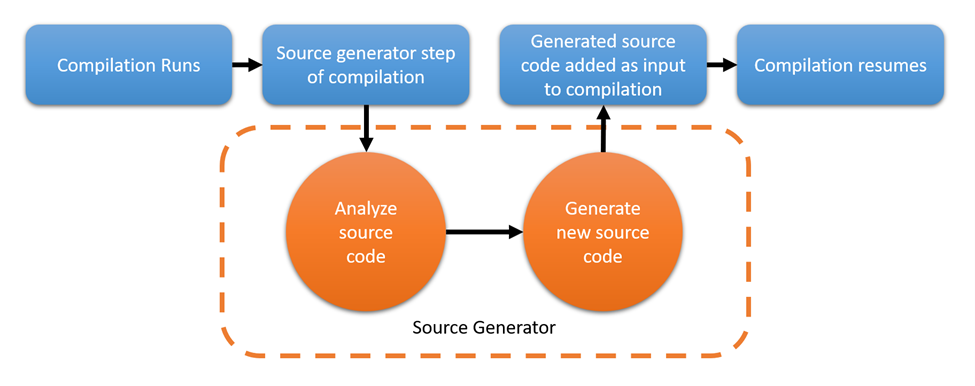
\includegraphics[width=\linewidth]{graphics/source-generator-visualization.png}
\caption{An overview of the C\# source generators workflow.}
\label{fig:source_generators_overview}
\end{figure}

The primary steps involved in the functionality of C\# source generators, as illustrated in Figure \ref{fig:source_generators_overview}, are code analysis, code generation, and integration. In the code analysis step, the source generator examines the syntax tree and semantic model, which are hierarchical representations of the source code. Analyzing these structures enables the source generator to understand the structure and relationships within the code, paving the way for generating meaningful and contextually relevant source code.

For example, a source generator could analyze a codebase and detect a common pattern, such as logging messages throughout the application. Based on this analysis, it could then generate a centralized logging class that captures all logging-related information, making the logging process more consistent and maintainable.

Once the analysis is complete, the source generators create new source code based on the previous analysis. This integration between analysis and generating source code allows the source generator to create custom code tailored to the application's specific needs. The generated code can range from complete class or method definitions to partial implementations that complement existing code. For instance, a source generator could generate a custom serializer for a specific data type, reducing the overhead associated with runtime reflection and improving serialization performance.

Finally, during compilation, the generated code is seamlessly integrated into the existing codebase to ensure it works harmoniously with the rest of the application. This crucial aspect of source generators allows developers to take advantage of their power without interrupting their current development processes, as generated code can be easily integrated into existing codebases.

\subsection{Exploring Syntax Trees and Semantic Models in Source Generators}

An Abstract Syntax Tree (AST) is a hierarchical representation of the syntactic structure of source code. It abstracts away the concrete syntax details, such as punctuation and whitespace, and focuses on the relationship between code elements, such as variables, methods, and classes. Figure \ref{fig:ast_example} provides a visualization of an AST, illustrating how code elements are organized into a tree structure. ASTs are essential for compilers and other code analysis tools, as they provide a structured representation of the code that can be more easily manipulated and analyzed.

\begin{figure}[H]
    \centering
    \begin{adjustbox}{max width=\textwidth, max height=0.51\textheight, keepaspectratio}
        \includesvg{graphics/Abstract_syntax_tree_for_Euclidean_algorithm.svg}
    \end{adjustbox}
    \caption{Example of an Abstract Syntax Tree}
    \label{fig:ast_example}
\end{figure}

ASTs enable source generators to analyze and manipulate code during the compilation process. As shown in Figure \ref{fig:ast_example}, source generators can gather information about the code structure and identify patterns by traversing the AST. This information is then used to generate new source code that addresses the specific goals set by the programmer, whether it be enhancing existing code or creating entirely new functionality. The flexibility provided by ASTs enables developers to achieve their desired outcomes.

Source generators use the .NET Compiler Platform (Roslyn) to access and manipulate ASTs. Roslyn provides rich APIs that enable developers to examine, analyze, and modify ASTs efficiently. For example, a source generator can traverse an AST to find all classes implementing a specific interface or search for specific method invocations within the code.

Understanding the structure and properties of ASTs, along with the APIs provided by Roslyn, is helpful for developers working with source generators. ASTs consist of key elements such as nodes, tokens, and trivia. Nodes symbolize the primary syntactic constructs, like statements and expressions, while tokens constitute the terminal elements of the syntax, including keywords, identifiers, and literals. Trivia represents non-essential syntax elements, such as comments and whitespace. Through the Roslyn APIs, developers can navigate and manipulate the AST, conduct various code analysis tasks, and create new source code based on the analysis results.

The process generally encompasses the following steps:
\begin{itemize}
\item Obtaining the syntax tree for the code being compiled.
\item Traversing the syntax tree to identify specific code elements, patterns, or relationships.
\item Analyzing the AST to collect structural information and detect potential optimizations.
\item Generating new source code based on the analysis results.
\item Integrating the generated code into the existing codebase during compilation.
\end{itemize}

\subsection{Developing Source Generators}

Developers must adhere to several formal requirements when creating a functioning source generator using C\# source generators. These requirements include implementing the \texttt{ISourceGenerator} interface, initializing the generator, and registering syntax notifications. In addition, developers should be aware of the use of partial classes and their role in integrating the generated code.

\begin{enumerate}

\item \textbf{Adding Required References in the \texttt{.csproj} File:}\
Before implementing a source generator, the necessary references must be added to the project's \texttt{.csproj} file. These references include the \texttt{Microsoft.CodeAnalysis.CSharp.Workspaces} package provides the required APIs for working with C\# syntax trees, semantic models, and other code analysis components. Additionally, the \texttt{Microsoft.CodeAnalysis.Analyzers} package should be added to ensure adherence to best practices and conventions when developing source generators. To include these packages, add the following \texttt{PackageReference} elements to the \texttt{ItemGroup} section of the \texttt{.csproj} file:

\begin{listing}[H]
\begin{minted}{xml}
<ItemGroup>
    <PackageReference 
        Include="Microsoft.CodeAnalysis.CSharp.Workspaces" 
        Version="4.5.0" />
    <PackageReference 
        Include="Microsoft.CodeAnalysis.Analyzers" 
        Version="3.3.4" />
</ItemGroup>
\end{minted}
\caption{Adding required package references to the \texttt{.csproj} file for source generator development}
\end{listing}

One can implement the source generator with the required references by following the subsequent steps.

\item \textbf{Implementing the \texttt{ISourceGenerator} Interface and Applying the \texttt{Generator} Attribute:}\
A source generator must implement the \texttt{ISourceGenerator} interface, which defines two methods: \texttt{Initialize} and \texttt{Execute}. The \texttt{Initialize} method is called by the compiler when the source generator is first loaded. In contrast, the \texttt{Execute} method is invoked during the compilation process to generate new source code. Moreover, the source generator class must be decorated with the \texttt{[Generator]} attribute. This attribute indicates to the compiler that the class should be treated as a source generator, allowing the compiler to discover and load the generator at runtime.

\item \textbf{Initializing the Generator:}\\
The \texttt{Initialize} method of a source generator receives a \texttt{GeneratorInitializationContext} instance as a parameter. This context object allows the source generator to configure itself and register for specific notifications from the compiler, such as syntax node changes. Typically, a source generator will register for syntax notifications in the \texttt{Initialize} method using the \texttt{RegisterForSyntaxNotifications} method on the context object.

\item \textbf{Registering Syntax Notifications:}\\
To receive notifications about syntax nodes in the code being compiled, a source generator must provide an implementation of the \texttt{ISyntaxReceiver} interface. This interface defines a single method, \texttt{OnVisitSyntaxNode}, which the compiler calls for each syntax node in the code. The source generator can analyze these nodes and collect relevant information, such as candidate classes or methods for code generation. This step is optional if the source generator does not require information about the project code.

\item \textbf{Using Partial Classes:}\\
Source generators often rely on partial classes to integrate the generated code with the existing codebase. By marking a class as \texttt{partial}, the developer indicates that its implementation may be split across multiple files. This allows the source generator to generate new code in separate files combined with the original class during compilation. This approach ensures that the generated code does not interfere with the original source code and that the changes introduced by the generator can be isolated and easily managed.

\end{enumerate}

By adhering to these formal requirements, developers can create source generators that operate seamlessly within the C\# compiler and .NET ecosystem, allowing for powerful code generation and manipulation capabilities. Here is a simple example of a source generator that generates a "Hello, World!" method in a target class. This example will illustrate the key aspects of source generator development discussed above. We will break the example code into smaller chunks and explain each part individually.

The first step is to implement the \texttt{ISourceGenerator} interface. In this example, the \texttt{HelloWorldGenerator} class implements the interface, and the \texttt{Initialize} and \texttt{Execute} methods are defined:

\begin{listing}[H]
\begin{minted}{csharp}
[Generator]
public class HelloWorldGenerator : ISourceGenerator
{
    public void Initialize(GeneratorInitializationContext context)
    {
        context.RegisterForSyntaxNotifications(() => new SyntaxReceiver());
    }

    public void Execute(GeneratorExecutionContext context)
    {
        // Main source generator logic goes here
    }
}
\end{minted}
\caption{Implementing the \texttt{ISourceGenerator} interface}
\end{listing}

The \texttt{SyntaxReceiver} class is a custom implementation of the \texttt{ISyntaxReceiver} interface. It collects target classes marked with the \texttt{partial} keyword. The \texttt{OnVisitSyntaxNode} method is called for each syntax node in the compilation, and it adds class declarations with the \texttt{partial} modifier to the \texttt{CandidateClasses} list:

\begin{listing}[H]
\begin{minted}{csharp}
private class SyntaxReceiver : ISyntaxReceiver
{
    public List<ClassDeclarationSyntax> CandidateClasses { get; } = new();
    
    public void OnVisitSyntaxNode(SyntaxNode syntaxNode)
    {
        if (syntaxNode is ClassDeclarationSyntax classDeclaration 
            && classDeclaration.Modifiers.Any(SyntaxKind.PartialKeyword))
        {
            CandidateClasses.Add(classDeclaration);
        }
    }
}
\end{minted}
\caption{Implementing the SyntaxReceiver class}
\end{listing}

Let's move on to the \texttt{Execute} method. This is where the main logic of the source generator is implemented. The generator checks if the \texttt{SyntaxReceiver} instance is available and then iterates through the collected \texttt{CandidateClasses}. For each target class, it generates the "Hello, World!" method and adds it to the existing class using a \texttt{StringBuilder}:

\begin{listing}[H]
\begin{minted}{csharp}
public void Execute(GeneratorExecutionContext context)
{
    if (context.SyntaxReceiver is SyntaxReceiver receiver)
    {
        foreach (var classDeclaration in receiver.CandidateClasses)
        {
            var className = classDeclaration.Identifier.Text;
            var namespaceName = 
                (classDeclaration.Parent as NamespaceDeclarationSyntax)?
                    .Name.ToString() ?? "Global";
            
            var sourceBuilder = new StringBuilder($@"
namespace {namespaceName}
{{
    partial class {className}
    {{
        public void HelloWorld()
        {{
            Console.WriteLine(""Hello, World!"");
        }}
    }}
}}
");
            context.AddSource($"{className}.g.cs", 
                SourceText.From(sourceBuilder.ToString(), Encoding.UTF8));
        }
    }
}
\end{minted}
\caption{Generating the "Hello, World!" method in the Execute method}
\end{listing}

The generated "Hello, World!" method is added to the target class within its namespace. The generator then calls the AddSource method, passing a unique identifier and the source text. The generated code is integrated into the existing codebase during the compilation process.

In the following example, we have a simple partial class:

\begin{listing}[H]
\begin{minted}{csharp}
namespace SourceGeneratorExample
{
    public partial class PartialClassTest { }
}
\end{minted}
\caption{Source code of the example partial class}
\end{listing}

After the source generator is executed, it adds a \texttt{HelloWorld} method to the \texttt{PartialClassTest} class, resulting in the following generated code:

\begin{listing}[H]
\begin{minted}{csharp}
namespace SourceGeneratorExample
{
    partial class PartialClassTest
    {
        public void HelloWorld()
        {
            Console.WriteLine("Hello, World!");
        }
    }
}
\end{minted}
\caption{Generated code for the example partial class with the HelloWorld method}
\end{listing}

\subsection{Limitations and Challenges of Using C\# Source Generators}

Despite their numerous benefits, C\# source generators have some limitations and challenges associated with their use. This section discusses some of the main concerns and potential pitfalls developers might face when working with source generators.

One significant limitation of source generators is their inability to modify existing code\cite{Microsoft2022SourceGenerators}. Source generators can only add new code to the compilation process, not change or remove existing code. This constraint may make it difficult for developers to refactor or optimize existing codebases using source generators. Developers must work around this limitation by using partial classes and methods or by designing their applications with source generators in mind from the beginning\cite{Bolognese2021UsingBlog}.

Another challenge with source generators is the learning curve of understanding the .NET Compiler Platform (Roslyn) and its APIs\cite{MicrosoftThePlatform}. While Roslyn provides a powerful set of APIs for code analysis and transformation, developers may need significant time and effort to become proficient with these tools. Additionally, the documentation for Roslyn and its APIs can be overwhelming for developers who are new to the technology\cite{Microsoft2021TheLearn}.

The performance of source generators can also be a concern, as the generation process adds overhead to the compilation time\cite{Microsoft2022SourceGenerators}. While the generated code can improve runtime performance, the increased compilation time may lead to a slower development experience. Developers should be mindful of this trade-off and consider the potential impact on their development workflows.

Error handling and debugging in source generators can be challenging, as the generated code may introduce new bugs or unexpected behavior\cite{Microsoft2022SourceGenerators}. Diagnosing issues in the generated code may be difficult, as developers need to examine both the source generator code and the generated code to identify the root cause of the problem. To alleviate this issue, some best practices, such as providing clear error messages and generating debuggable code, should be followed\cite{Bolognese2021UsingBlog}.

Finally, adopting source generators can introduce additional complexity to the build process and tooling\cite{Microsoft2022SourceGenerators}. Integrating source generators into existing build systems may require additional configuration, and developers must ensure that their tooling supports the generation process. As source generators become more widely adopted, tooling and build systems are expected to evolve and improve to accommodate their use better.

\section{Reflection in Software Development}

\begin{itemize}
    \item Definition of reflection and its role in software development
    \item Explanation of how reflection is used
\end{itemize}

\subsection{Concepts and Principles}

\begin{itemize}
    \item Key concepts and principles of reflection
    \item How reflection interacts with code at runtime
\end{itemize}

\subsection{Performance Implications}

\begin{itemize}
    \item Impact on reflection on performance
    \item Trade-offs and challenges related to reflection usage
\end{itemize}

\section{Code Generation Techniques}

\begin{itemize}
    \item Overview or various code generation techniques e.g. T4
    \item Comparison between static and runtime code generation
    \item Advantages and disadvantages of different approaches
\end{itemize}

\section{Related Work and Studies}

Using C\# source generators has received little attention in the existing research. While a few books \cite{Franz2022TrendsCompilerbau, Microsoft2022SourceGenerators, Vermeir2022.NETPlatform} are available on the implementation of C\# source generators and their integration in Roslyn; the official documentation \cite{Microsoft2022SourceGenerators} is lacking in detail. There are some papers on C\# source generators. However, they focus on the potential use cases and a general understanding of the feature \cite{Slimak2022SourceSLIMAK}. Conversely, this bachelor thesis will focus on the possible performance gain when using C\# source generators for reflected code.

Research on the performance penalty of reflective code in general and other programming languages is widely available. There have been various studies \cite{Forman2005EvaluatingPerformance, Halloway2001ReflectionInformIT, JavaReflection2013} which measure the performance of reflection in Java applications. In some of these studies, it has been explicitly stated that the development speed gained from using reflection outweighs the performance hit \cite{Halloway2001ReflectionInformIT}. However, with the rise of globalization and the need to process millions of user requests as fast as possible, every possible performance gain becomes crucial. Regardless of the development speed, all reviewed studies concluded that reflection imposes a significant performance penalty \cite{Forman2005EvaluatingPerformance, Halloway2001ReflectionInformIT, JavaReflection2013}. Therefore, it is important to investigate alternative approaches to mitigate this penalty.

This bachelor thesis aims to contribute to software engineering and performance optimization by investigating the potential benefits of using C\# source generators for reflected code. The existing research on reflection \cite{Forman2005EvaluatingPerformance, Halloway2001ReflectionInformIT, JavaReflection2013} mostly focuses on Java, which makes it difficult to determine the potential gains for C\#. Therefore, we aim to fill this gap in the literature by conducting a controlled experiment and comparing the observed runtime performance to the existing research. The results will provide a deeper understanding of the trade-off between build time and runtime performance in C\# applications. By doing so, we hope to provide useful insights for developers who strive to balance performance and development time in their applications.

